
%(BEGIN_QUESTION)
% Copyright 2015, Tony R. Kuphaldt, released under the Creative Commons Attribution License (v 1.0)
% This means you may do almost anything with this work of mine, so long as you give me proper credit

Solenoid valve SV-92 plays an important role in this compressor inlet separator control system.  Level control valve LV-92 opens up when needed to drain liquid out of the ``boot'' of the separator vessel, which ideally contains only gas (vapor).  Examine this P\&ID and then answer the following questions:

$$\includegraphics[width=15.5cm]{i0003rx01.eps}$$

\begin{itemize}
\item{} Identify the statuses of SV-92 and LV-92 when the separator boot liquid level is at or below the normal level of 1 foot 4 inches.
\vskip 10pt
\item{} Describe how this system responds to high liquid levels in the separator boot.
\vskip 10pt
\item{} What will be the consequence of an instrument air supply failure, as it relates to the separator boot liquid level?
\vskip 10pt
\item{} What will be the consequence of an AC power failure to LIC-92?
\end{itemize}

\underbar{file i00953}
%(END_QUESTION)





%(BEGIN_ANSWER)

\begin{itemize}
\item{} Identify the statuses of SV-92 and LV-92 when the separator boot liquid level is at or below the normal level of 1 foot 4 inches.  {\it LV-92 will be closed, and SV-92's coil will be de-energized.}
\vskip 10pt
\item{} Describe how this system responds to high liquid levels in the separator boot.  {\it If LT-92 senses a high liquid level, controller LIC-92 will respond by applying electrical power to SV-92.  When SV-92 actuates, it sends instrument air to the diaphragm actuator of LV-92 to cause that drain valve to open.  As LV-92 drains liquid out of the boot, the level sensed by LT-92 decreases over time, eventually to a point where controller LIC-92 stops sending power to the coil of SV-92.}
\vskip 10pt
\item{} What will be the consequence of an instrument air supply failure, as it relates to the separator boot liquid level?  {\it Without instrument air supply (IAS), the level drain valve LV-92 can never open and the separator boot liquid level will rise unabated.  Eventually LSHH-231 will detect the high-high level condition and command the Emergency Shut-Down (ESD) system to turn the compressor off in order to avoid damaging that machine.}
\vskip 10pt
\item{} What will be the consequence of an AC power failure to LIC-92?  {\it Without AC power to energized the coil of solenoid SV-92, the level drain valve LV-92 will never be commanded to open by SV-92 and the separator boot liquid level will rise unabated.  Eventually LSHH-231 will detect the high-high level condition and command the Emergency Shut-Down (ESD) system to turn the compressor off in order to avoid damaging that machine.}
\end{itemize}


%(END_ANSWER)





%(BEGIN_NOTES)


%INDEX% Final Control Elements, valve: fail-safe solenoids
%INDEX% Process: gas compressor inlet separator (realistic P&ID shown)

%(END_NOTES)


